\documentclass[10pt]{article}
\usepackage[utf8]{inputenc}
\usepackage[T1]{fontenc}
\usepackage{amsmath}
\usepackage{amsfonts}
\usepackage{amssymb}
\usepackage[version=4]{mhchem}
\usepackage{stmaryrd}
\usepackage{graphicx}
\usepackage[export]{adjustbox}
\graphicspath{ {./images/} }
\usepackage{bbold}

\DeclareUnicodeCharacter{21D2}{\ifmmode\Rightarrow\else{$\Rightarrow$}\fi}

\begin{document}
$(R P): V(k)=\max _{k^{\prime} \in \Gamma(k)}\left\{F\left(k, k^{\prime}\right)+\beta V\left(k^{\prime}\right)\right\}$\\
Trecivsive problem k'erik)\\
Does ( $R P$ ) have a unique solution.?\\
Observe the structure of 1t:\\
RHS: transforms $V(k)$ into sometuing else by applying the max function\\
LHS: Just $V(k)$ by itself\\
Denote the RHS of (RP) by "operator"

$$
T V(k)=\max _{k^{\prime} \in T(k)}\left\{F\left(k, k^{\prime}\right)+\beta V\left(k^{\prime}\right)\right\}
$$

$\Rightarrow(R P)$ becomes $\quad V=T V$,\\
i.e. $V$ is the "fixed point" of operator $T$\\
Thus (RP) has a unique solution if and only if operator $T$ has a unique fixed point.

Under some conditions, $T$ is a "contractron mapping" $\Rightarrow \exists$ ! (there exists unique) gixed pornt.

Graphical interition:\\
$S$ - space of possible functrons V\\
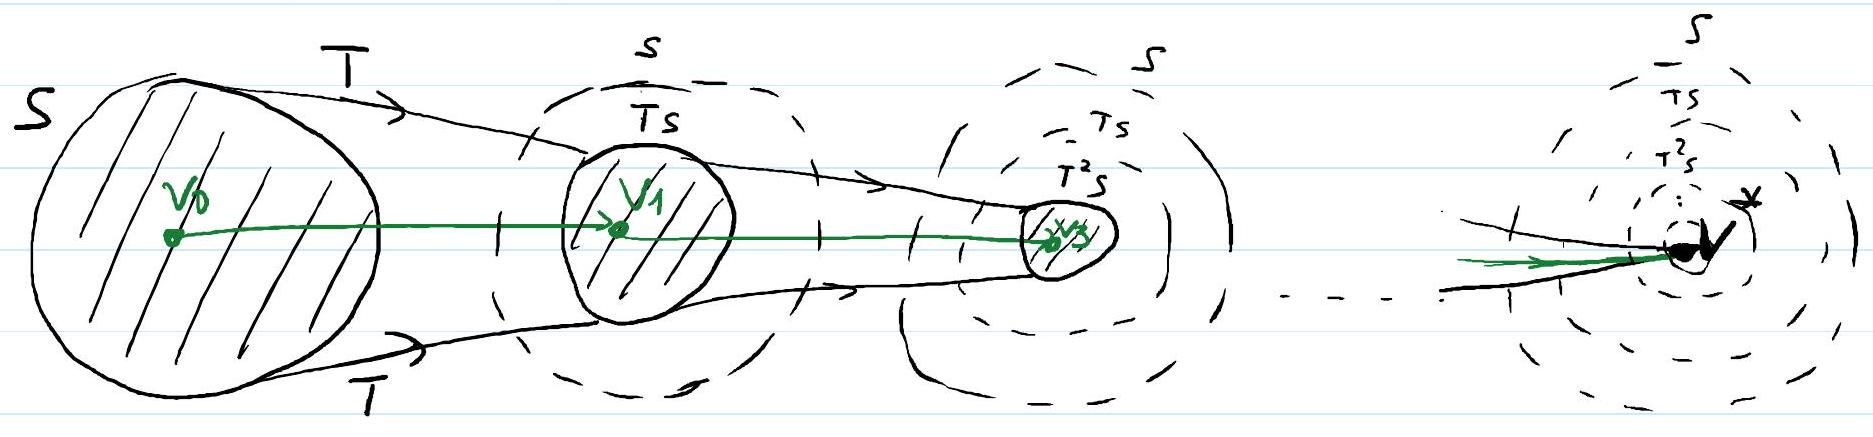
\includegraphics[max width=\textwidth, alt={}, center]{61ceb9f0-80e6-4a88-adcd-aedde3edbc6b-1_437_1873_2086_247}

\begin{itemize}
  \item If $T$ is a "contraction" ( ± maps a space into its interior) $\Rightarrow 7!$ fixed point $V^{*}$ that maps into itself:
\end{itemize}

$$
V^{*}=T V^{*}
$$

\begin{itemize}
  \item This fixed point can be found by taking any $V_{0} \in S$, and applying $T$ to it infinitely many tomes.
\end{itemize}

Next, letts develop a rigorous argument supporting thers "intrition".

\section*{: Doold (Metric space)}
A metric space $(S, d)$ is ast $S$ and a metric (distand function) $d: s^{2} \rightarrow \mathbb{R}_{+}$such that:\\
(i) strict positivity: $\forall x, y \in S: d(x, y) \geq 0$," $=$ "iff $x=y$\\
(ii) symmetty: $\forall x, y \in S: d(x, y)=d(y, x)$\\
(iii) triangle inequality: $\forall x, y, z \in S: \quad d(x, y) \leq d(x, z)+d(z, y)$

Note: (i)-(iii) are the basic properties of Eucledean distance Example: $d(x, y)=\sup _{t \in \mathcal{R}}|x(t)-y(t)|$

\section*{Df (Cauchey sequence) (s.d)}
A sequence $\left\{x_{n}\right\}_{n=0}^{\infty}$ in a metric space ${ }^{V}$ is a Cauchey segrence if Cauchey sequence iff $\forall \varepsilon>0 \exists N \in \mathbb{R}_{+}: \forall n, m>N \quad d\left(x_{n}, x_{m}\right)<\varepsilon$

\section*{Df (a Complete Metric Space)}
A metric space is complete if each Cauchey sequence converges to a limit in the mettric space

\section*{Df (Contractron) $T: S \rightarrow S$}
An operator is a contraction iff $\exists \gamma \in[0,1): \forall x_{1}, x_{2} \in S d\left(T\left(x_{1}\right), T\left(x_{2}\right)\right) \leqslant \gamma d\left(x_{1}, x_{2}\right)$.\\
Here $\gamma$ is called "the moderlus".

\section*{Theorem: (Contraction Mapping)}
Suppose that $(S, d)$ is a complete metric space and $T: S \rightarrow S$ is a contraction of modulus $\gamma$.\\
Then:

\begin{itemize}
  \item $\exists!\hat{x} \in S: T(\hat{x})=\hat{x} \quad$ (unique fixed port)
  \item $\forall x_{0} \in S \quad\left\{T^{n}\left(x_{0}\right)\right\}_{n=1}^{\infty}$ converges to $\hat{x}$
\end{itemize}

\section*{Contraction Mapporng theorem}
Stated last time:

\section*{Theorem: (Contraction Mapping)}
Suppose that $(S, d)$ is a complete metric space and $T: S \rightarrow S$ is a contraction of modelus $\gamma$.

\section*{Then:}
$-\exists!\hat{x} \in S: T(\hat{x})=\hat{x} \quad$ (unique fixed pornt)

\begin{itemize}
  \item $\forall x_{0} \in S \quad\left\{T^{n}\left(x_{0}\right)\right\}_{n=1}^{\infty}$ converges to $x$
\end{itemize}

\section*{Proof:}
Steps: (1) Show that $\exists \lim _{n \rightarrow \infty} T^{n}\left(x_{0}\right)$ (ve. that $\left\{x_{n}\right\}_{n \geq 1}$ is a Canchey sequence)\\
(2) Show that $\hat{x}=\lim _{n \rightarrow \infty} x_{n}$ is a fixed point ( ⇒ J fixed point) ${ }^{n \rightarrow \infty}$\\
(3) Share that the fixed point is unique\\
(1) Need to show that $\forall \varepsilon \quad \exists N: \forall n, m>N: d\left(T^{n}\left(x_{0}\right), T^{m}\left(x_{0}\right)\right)<\varepsilon$ Let $m<n$

$$
\begin{aligned}
d\left(T^{n}\left(x_{0}\right), T^{m}\left(x_{0}\right)\right) & =d\left(T^{m}\left(T^{n-m}\left(x_{0}\right)\right), T^{m}\left(x_{0}\right)\right) \leqslant(T \text {-contract }) \\
& \leq \gamma^{m} d\left(T^{n-m}\left(x_{0}\right), x_{0}\right) \\
& =\gamma^{m} d\left(T^{n-m-1}\left(x_{1}\right), x_{0}\right) \leqslant \mid \text { triangle } \mid \leqslant \\
& \leqslant \gamma^{m} \cdot\left[d\left(T^{n-m-1}\left(x_{1}\right), T^{n-m-1}\left(x_{0}\right)\right)+d\left(T^{n-m-1}\left(x_{0}\right), x_{0}\right)\right]
\end{aligned}
$$

(I-contract.)

$$
\leqslant \gamma^{m} \cdot\left[\gamma^{n-m-1} d\left(x_{1}, x_{0}\right)+d\left(T^{n-m-2}\left(x_{1}\right), x_{0}\right)\right] \leqslant
$$

(triangle)

$$
\begin{aligned}
\leq \gamma^{m} \cdot\left[\gamma^{n-m-1} d\left(x_{1}, x_{0}\right)+d\right. & \left(T^{n-m-2}\left(x_{1}\right), T^{n-m-2}\left(x_{0}\right)\right)+ \\
& \left.+d\left(T^{n-m-2}\left(x_{0}\right), x_{0}\right)\right] \leqslant
\end{aligned}
$$

$\leqslant$ (contract) $\leqslant \gamma^{m} \cdot[\gamma^{n-m-1} d\left(x_{1}, x_{0}\right)+\gamma^{n-m-2} d\left(x_{1}, x_{0}\right)+\underbrace{d\left(T^{n-m-3}\left(x_{1}\right), x_{0}\right)}_{\text {apply the same steps }}] \leqslant 11$\\
$\leqslant \gamma^{m} \cdot\left[\gamma^{h-m-1}+\gamma^{h-m-2}+\gamma^{h-m-3}+\ldots+\gamma+1\right] \cdot d\left(x_{1}, x_{0}\right)$\\
$=\gamma^{m} \cdot \frac{1-\gamma^{n-m}}{1-\gamma} d\left(x_{1}, x_{0}\right) \leq \varepsilon$ for $m$ sufficiently large.\\
$\Rightarrow\left\{T^{n}\left(x_{0}\right)\right\}$ is a Couchey sequence\\
(2) Let $\hat{x}=\lim _{n \rightarrow \infty} T^{n}\left(x_{0}\right)$. Weed to show that $d(\hat{x}, T(\hat{x}))=0$ (by completeness of $(S, d)$ )

$$
\begin{aligned}
& d(\hat{x}, T(\hat{x})) \leq d\left(\hat{x}, T^{n}\left(x_{0}\right)\right)+d\left(T^{n}\left(x_{0}\right), T(\hat{x})\right) \\
& \quad \text { triangle } \\
& \text { T-contract. } \underset{\rightarrow}{d} \leqslant \underbrace{d\left(\hat{x}, T^{n}\left(x_{0}\right)\right)}_{\rightarrow 0, n \rightarrow \infty}+\gamma \underbrace{d\left(T^{n-1}\left(x_{0}\right), \hat{x}\right)}_{\rightarrow 0, n \rightarrow \infty} \\
& \Rightarrow d(\hat{x}, T(\hat{x}))=0
\end{aligned}
$$

(3) $\hat{x}$ is a unique fixed point\\
(i.e. $T^{n}\left(x_{0}\right)$ converges to the same $\hat{x}$ from any $x_{0}$ )

By contradiction:\\
supprose there is another fixed pount $\hat{y}$

$$
\begin{aligned}
\Rightarrow d(\hat{x}, \hat{y}) & \leqslant \underbrace{d(\hat{x}, \Gamma(\hat{x}))}_{=0}+d(T(\hat{x}), T(\hat{y}))+\underbrace{d(T(\hat{y}), \hat{y})}_{=0} \\
& \leqslant(\text { contraction }) \leqslant \gamma d(\hat{x}, \hat{y}) \\
\Rightarrow d(\hat{x}, \hat{y}) & =0
\end{aligned}
$$

Thus, we need to check that the operator $T$ (in the RHS of the Bellman Equation) is a contraction.\\
Namely, if $V, W$ are two functions then $d(T(V), T(W)) \leq \gamma d(V, W)$ for some $\gamma<1$

So we need to define metric $d$ and, possibly, impose a restriction on the set of functions.

Let's use the sup norm

$$
\begin{aligned}
\|V\| & =\sup _{k \in X}|V(k)| \quad \text { where } X \text { is the set on which } \\
d(V, W) & =\|V-W\|=\sup _{k \in x}|V(k)-W(k)|
\end{aligned}
$$

For this metric to be well-defined, $V$ \& $W$ must be bounded.

The following result establishes sufficient conditions under which operator $T$ in the metric specce of (bounded functrons, sup norm) is a contraction:

\section*{Theorem: Blackwell's Sufficient Condition}
Let $B(X)$ be a set of bounded functions on $X$, and suppose that $T: B \rightarrow B$ satisfies

\begin{enumerate}
  \item Monotonicity: $\forall V, W \in B(X): V \leq W \Rightarrow T(V) \leq T(W)$
  \item Discounting: $\exists \forall \in[0,1): \forall c \in \mathbb{R}_{+} \quad \forall V \in B(x)$
\end{enumerate}

$$
T(V+c) \leqslant T V+\gamma c
$$

Then $T$ is a contraction of modelus sup w.r.t. sup. metrics\\
Proof: Need to show that

$$
\sup _{k \in x} \mid\left(T V(k)-(T W)(k)\left|\leqslant \gamma \sup _{k \in X}\right| V(k)-W(k) \mid\right.
$$

$\forall k: V(k)=W(k)+[V(k)-W(k)]$

$$
\leq w(k)+\sup _{k}|V(k)-w(k)|=w(k)+d(V, w)
$$

Monotonicity $\Rightarrow \quad T V \leq T(W+\underbrace{d(V, W)}_{\text {constant }}) \leqslant /$ discounting/

$$
\leq T w+\gamma \cdot d(V, w)
$$

$\Rightarrow T V-T W \leq \gamma \cdot d(V, W)$\\
Likewise, $W(k)=V(k)+[W(k)-V(k)]$\\
.... Same arguments ...\\
⇒ $\quad T W-T V \leq \gamma \cdot d(W, V)=\gamma \cdot d(V, W)$ (symmetry of $d(V, W)$ )\\
$\Rightarrow \quad-\gamma \cdot d(V, W) \leq T V-T W \leq \gamma \cdot d(V, W)$

$$
\begin{aligned}
\Rightarrow \sup _{k}|(T V)(k)-T W(k)| \leqslant & \gamma \cdot d(V, W)= \\
& \gamma \cdot \sup _{k}|V(k)-W(k)|
\end{aligned}
$$


\end{document}